	
\documentclass[a4paper,12pt]{article} 
\usepackage{amsmath, amssymb}
\usepackage{kotex}
\usepackage{graphicx}
\usepackage[figuresright]{rotating} 

\begin{document} 

\title{과제3 보고서}
\author{B211103 변준석}
\date{2017년 10월}
\maketitle

\newpage
\section{개요}
이번 과제의 첫 번째 메인 프로그램인 \textsl{hw2a.cpp} 에서는 다항식을 디자인한 클래스의 덧셈 연산을 오버로딩하여 구현하였고 쉬프트 연산을 오버로딩하여 다항식 클래스들을 입출력할 수 있게 만들었다.
두 번째 메인 프로그램인 \textsl{hw2b.cpp} 에서는 추가적으로 곱셈 연산까지 오버로딩하여 구현하였다.

\section{문제 해결 방안}
이번 과제의 다항식의 클래스를 구현함에 있어서 효율적인 데이터 사용을 위해 계수가 0인 항들은 저장하지 않았으며, 실제 저장한 항의 개수인 \textsl{terms}변수와 다항식의 변수인 텀 클래스 배열의 크기를 \textsl{capacity}변수로 저장하였다.
다항식의 출력은 최고차항 순으로 항을 정렬하였으며, 계수와 차수에 따라 출력하는 형태가 달라진다. 계수와 차수에 따라 다른 출력 알고리즘을 갖고 있다. 덧셈은 연산이 다 끝났을 때 결과 클래스의 텀 배열이 최고차항부터 저장되도록 하였다.
곱셈연산은 실제로 우리가 다항식의 곱셈 계산을 어떤 방식으로 하는 지 고려하여 룹을 만들었다. 곱셈 연산에서 중간결과들을 다항식 클래스의 배열로 동적 할당하여 이 모든 중간결과들을 더했다. 이로써 추가적인 항 저장의 순서 정렬 필요없이 최고차항부터 저장된 결과값을 얻을 수 있다.


\section{hw2b의 곱셈 구현}
곱셈의 구현은 의외로 간단하게 해결하였다. 덧셈에서 결과물을 최고차항 순으로 저장하는 알고리즘을 갖고있기 때문에 이를 그대로 이용하여 간단하게 구현할 수 있었다.
곱셈 오버로딩 함수의 중간에서 \textsl{Polynomial}클래스의 배열을 그 클래스의 \textsl{terms}변수의 크기로 동적 할당하였다. 그 결과물이 \textsl{t}이다.
첫 번째 \textsl{t[0]}에 저장되는 다항식은 \textsl{p1}의 첫 번째 항과 \textsl{p2}전체의 곱이다. \textsl{t[n]}에 저장되는 다항식은 \textsl{p1}의 \textsl{n+1}번째 항과 \textsl{p2}전체의 곱이다.
배열\textsl{t}의 모든 다항식을 더하였을 때 \textsl{p1}과 \textsl{p2}의 결과가 도출된다. 결과를 도출하는 마지막 과정에서 \textsl{hw2a}에서 오버로딩한 덧셈을 사용하였기 때문에 그 결과는 최고차항 순으로 저장된 \textsl{termArray}를 갖고 있다.


\section{최종 출력 hw2a}
3x\^{}5 +2x\^{}3 -4
\newline
x\^{}8 -7x\^{}5 -x\^{}3 -3
\newline
x\^{}8 -4x\^{}5 +x\^{}3 –7

\section{hw2a의 간단한 설명}
최종 출력의 첫 번째 줄에서는 \textsl{p1}이 쉬프트 연산자 오버로딩을 통해 제대로 출력된 것을 확인할 수 있었다.
두 번째 줄에서는\textsl{p2}가 쉬프트 연산자 오버로딩을 통해 제대로 출력된 것을 확인할 수 있었다.
마지막 줄에서는 \textsl{p1}과 \textsl{p2}의 합인 \textsl{p3}가 제대로 연산되어 최고차항 순으로 출력된 것을 확인할 수 있었다.


\section{최종 출력 hw2b}
3x\^{}5+2x\^{}3-4
\newline
x\^{}8-7x\^{}5-x\^{}3-3
\newline
3x\^{}13+2x\^{}11-21x\^{}10-21x\^{}8-2x\^{}6+19x\^{}5-2x\^{}3+12

\section{hw2b의 간단한 설명}
최종 출력의 첫 번째 줄에서는 \textsl{p1}이 쉬프트 연산자 오버로딩을 통해 제대로 출력된 것을 확인할 수 있었다.
두 번째 줄에서는\textsl{p2}가 쉬프트 연산자 오버로딩을 통해 제대로 출력된 것을 확인할 수 있었다.
마지막 줄에서는 \textsl{p1}과 \textsl{p2}의 곱인 \textsl{p3}가 제대로 연산되어 최고차항 순으로 출력된 것을 확인할 수 있었다.


\newpage
\begin{figure}[t]\vspace*{4pt} 
\centerline{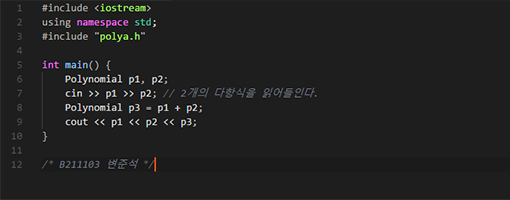
\includegraphics[width=1.0\columnwidth]{hw2a}} 
\caption{hw2a.cpp}\vspace*{-6pt} 
\label{figure:hw2a} 
\end{figure} 

\begin{figure}[t]\vspace*{4pt} 
\centerline{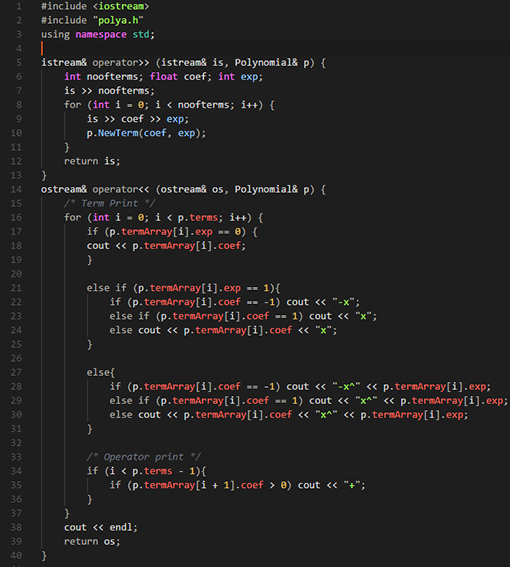
\includegraphics[width=1.0\columnwidth]{polya1}} 
\caption{polya.cpp의 쉬프트 연산 오버로딩}\vspace*{-6pt} 
\label{figure:polya1} 
\end{figure} 

\begin{figure}[t]\vspace*{4pt} 
\centerline{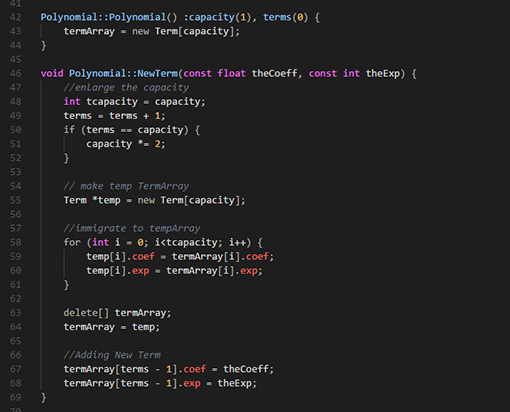
\includegraphics[width=1.0\columnwidth]{polya2}} 
\caption{polya.cpp의 클래스 생성자와 항 추가 함수}\vspace*{-6pt} 
\label{figure:polya2} 
\end{figure} 

\begin{figure}[t]\vspace*{4pt} 
\centerline{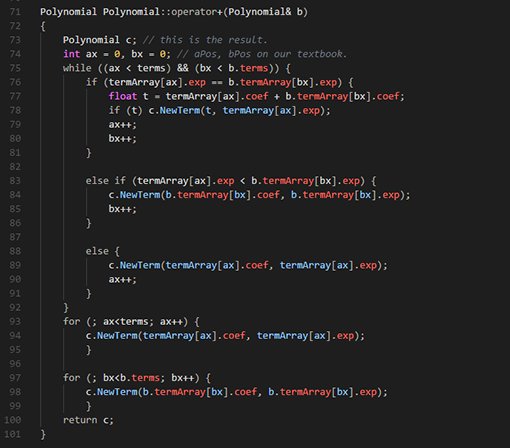
\includegraphics[width=1.0\columnwidth]{polya3}} 
\caption{polya.cpp의 다항식 덧셈 오버로딩}\vspace*{-6pt} 
\label{figure:polya3} 
\end{figure} 


\begin{figure}[t]\vspace*{4pt} 
\centerline{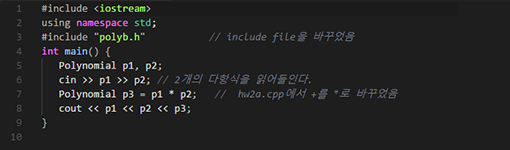
\includegraphics[width=1.0\columnwidth]{hw2b}} 
\caption{hw2b.cpp}\vspace*{-6pt} 
\label{figure:rawdata} 
\end{figure} 

\begin{figure}[t]\vspace*{4pt} 
\centerline{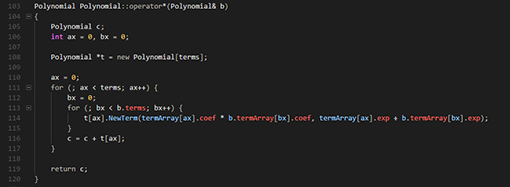
\includegraphics[width=1.0\columnwidth]{polyb}} 
\caption{polyb.cpp의 다항식 곱셈 오버로딩}\vspace*{-6pt} 
\label{figure:rawdata} 
\end{figure} 


\end{document} 